
%% Beamer poster theme created for Imperial College by LianTze Lim
%% LICENSE: LPPL 1.3
\documentclass[xcolor={table}]{beamer}
\usepackage[size=a0,orientation=landscape,scale=1.55]{beamerposter}
\setlength{\oddsidemargin}{1in}
\usepackage{wrapfig}
\usepackage{amsmath}
\usepackage{tabu}
\usepackage{booktabs}
%\usepackage{subcaption}
\usepackage[caption=false]{subfig}
% \captionsetup[table]{font={stretch=1.2}}     %% change 1.2 as you like

\newcommand{\arxiv}[1]{}

\usetheme{ImperialPoster}
%% Four available colour themes
\usecolortheme{ImperialWhite} % Default
% \usecolortheme{ImperialLightBlue}
% \usecolortheme{ImperialDarkBlue}
% \usecolortheme{ImperialBlack}

\title{Demystifying MMD GANs}
\author{
  \mainauthor{Miko{\l}aj Bi\'nkowski}\Tsup{1}, 
  \mainauthor{Dougal J. Sutherland}\Tsup{2},
  Michael Arbel\Tsup{2},
  Arthur Gretton\Tsup{2}
}
\institute{
  \Tsup{1}Department of Mathematics, Imperial College London \qquad
  \Tsup{2}Gatsby Computational Neuroscience Unit, University College London\\
  \texttt{\{mikbinkowski,dougal,michael.n.arbel,arthur.gretton\}@gmail.com}
}

\DeclareMathOperator{\D}{\mathcal{D}}
\DeclareMathOperator*{\E}{\mathbb{E}}
\newcommand{\F}{\mathcal{F}}
\newcommand{\h}{\mathcal{H}}
\DeclareMathOperator{\mean}{mean}
\newcommand{\PP}{\mathbb P}
\newcommand{\QQ}{\mathbb Q}
\newcommand{\R}{\mathbb R}
\DeclareMathOperator{\W}{\mathcal{W}}
\newcommand{\X}{\mathcal X}
\newcommand{\Z}{\mathcal Z}
\newcommand{\ZZ}{\mathbb Z}
\DeclareMathOperator*{\argmin}{argmin}
\DeclareMathOperator*{\argmax}{argmax}
\DeclareMathOperator{\mmd}{MMD}
\DeclareMathOperator{\FID}{FID}

\addbibresource{refs.bib}

\begin{document}
\addtobeamertemplate{headline}{} % Imperial Logo. This is a bit hacky
{
\begin{tikzpicture}[remember picture,overlay] 
\node [shift={(11cm,-5cm)}] at (current page.north west) {
\includegraphics[height=3cm]{Imperial_logo.pdf}}; 
\end{tikzpicture} 
\begin{tikzpicture}[remember picture,overlay]
\node [shift={(-10cm,-5cm)}] at (current page.north east) {
\includegraphics[height=7cm]{gatsby.jpg}};
\end{tikzpicture}
}

\begin{frame}{}
\maketitle
\begin{columns}[T, totalwidth=\textwidth]

  \begin{column}{.32\textwidth}
    \begin{block}{Overview}
      \begin{itemize}
        \item We relate the formulation of MMD GANs to Wasserstein and Cram\'er GANs
              via the notion of witness functions.
        \item We clarify the situation of gradient bias in optimizing GANs:
              ``outer loop'' gradients are biased, but update steps are unbiased.
        \item We propose a new measure of GAN performance, %the \emph{Kernel Inception Distance} and 
              and use it to adapt the learning rate during training.
      \end{itemize}
    \end{block}
    % \vspace*{-1.2cm}
    \begin{block}{Relation to Wasserstein and Cram\'er GANs} 
      Integral Probablity Metrics (IPMs) %form a family of divergences between 
      are distances between distributions
      defined by a class of \emph{critic} functions $\F$:
      \[
        \D(\PP, \QQ)
        = \sup_{f \in \F} \D_f(\PP, \QQ)
        = \sup_{f\in\F} \E_{X\sim\PP}[f(X)] - \E_{Y\sim\QQ}[f(Y)].
      \]

      \vspace*{-1.5ex}\begin{itemize}
        \item{\textbf{Wasserstein distance} has $\F$ the set of 1-Lipschitz functions
          \[  
            \F = \left\{f: \sup_{x,y} \frac{|f(x) - f(y)|}{\|x - y\|}\leq 1\right\}. 
          \]
          WGANs approximate $f$ with a critic network,
          using weight clipping \citep{wgan}
          or gradient penalty \citep{wgan-gp}.
        \item \textbf{Maximum Mean Discrepancy (MMD)} %\citep{mmd-jmlr}
          has $\F$ a unit ball in some 
          \emph{Reproducing Kernel Hilbert Space (RKHS)} $\h$ with kernel $k$
          \[ \F = \left\{f: \|f\|_{\h} \leq 1\right\}. \]
          MMD value and the optimal critic are known in closed form:
          \begin{align*}
            \mmd_k^2(\PP, \QQ) &= \E_{\PP} k(X,X') + \E_{\QQ} k(Y,Y') - 2\E_{\PP,\QQ} k(X,Y),\\
            f^*(t) &\propto \E_{\PP}k(X, t) - \E_{\QQ}k(Y, t).
          \end{align*}
        }
        \item
          MMD GANs \citep{mmd-gan} optimize \emph{representation} in kernel 
          \[ k_{\theta}(x, y) = k_\mathrm{base}(h_{\theta}(x), h_{\theta}(y)), \]
          corresponding to distance
          \[ \D(\PP, \QQ) = {\sup}_\theta \D_\theta(\PP, \QQ) = {\sup}_{\theta} \mmd_{k_\theta}^2(\PP, \QQ). \]
        \item Cram\'er GAN \citep{cramer-gan} is essentially an MMD GAN with the \emph{Energy Distance} kernel.
        \item WGANs are \emph{almost} an MMD GAN with linear $k_\mathrm{base}$.
      \end{itemize}

      Wasserstein and (Gaussian kernel) MMD witness functions: \\[1ex]
      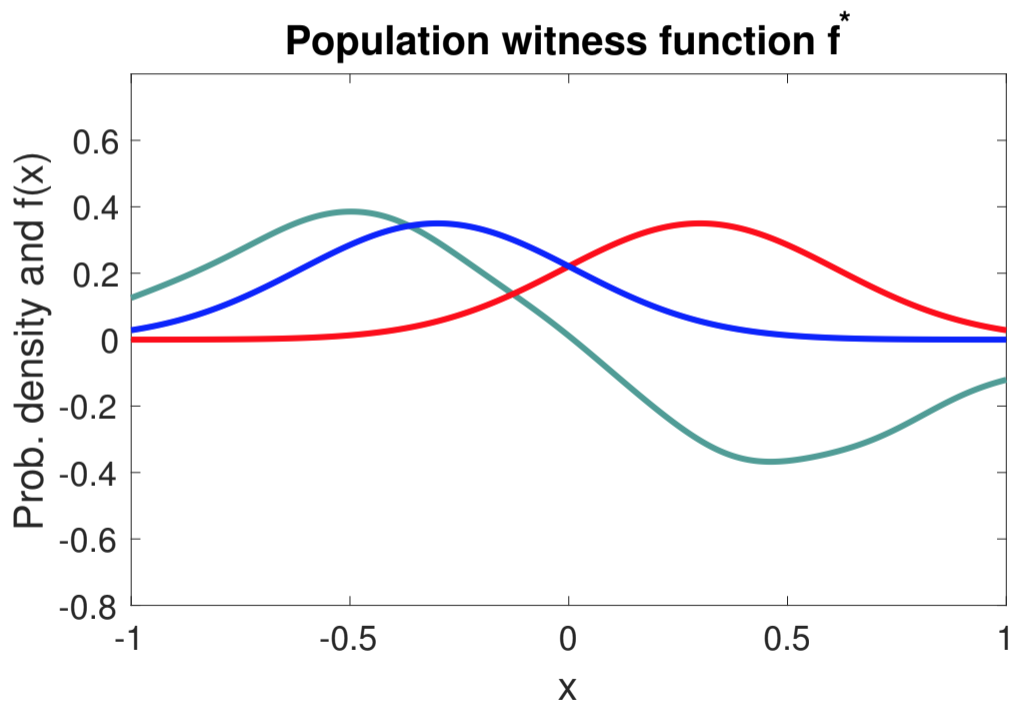
\includegraphics[width=\linewidth]{figs/witness.png}\\
      Note multiple sample-optimal Wasserstein critics (light blue).
    \end{block}
  \end{column}

  \begin{column}{.32\textwidth}
    \begin{block}{Gradient Penalty}
      Extending the idea of \citet{wgan-gp}, we penalize the
      gradient of the witness function in MMD GANs:
      \[ Loss^{critic}(\theta) = \widehat{\mmd}_{\theta}^2(\PP, \QQ_{\psi}) + \lambda\E_{\tilde{X}}\left(\|\nabla_{\tilde{X}} f^*(\tilde{X})\| - 1\right)^2. \]
      %where $\tilde{X}$ are drawn between points from $\PP$ and $\QQ_{\psi}$. %$\widehat{MMD}$ is an unbiased MMD estimator.% and $\QQ_{\psi} = G_{\psi}(\ZZ)$ is the generated distribution.
    \end{block}
    \vspace*{-1.3cm}
    \begin{block}{Theory: Biased gradient estimates}
      \citet{cramer-gan} claim that WGANs have biased gradients, while Cram\'er GANs do not. We show:
      \vspace*{-1.5ex}
      \begin{itemize}
        \item For a \emph{fixed kernel} (MMD GAN) or \emph{fixed critic} (WGAN),
              generator gradient steps are unbiased.
              (Same for critic.)
        \begin{itemize}
          \item General proof of $\E \nabla f = \nabla \E f$ for feedforward networks $f$.
        \end{itemize}
        \item ``Outer-loop'' gradient steps, $\nabla_\psi \hat\D(X, G_{\psi}(Z))$, are biased.
        \begin{itemize}
          \item Estimators with non-constant bias have biased gradients.
          \item Optimization-based estimators are biased:
            \[
            \E \hat\D(X, Y)
                 = \E \hat\D_{\hat f_{tr}}(X_{te}, Y_{te})
                 = \E \D_{\hat f_{tr}}(\PP, \QQ)
                 \le {\sup}_f \D_f(\PP, \QQ)
            .\]
          \item No possible unbiased estimator exists for IPMs $\D$.
          \item Small minibatch sizes \emph{don't} introduce bias: bias vanishes as critic becomes optimal.
        \end{itemize}
      \end{itemize}
    \end{block}
    \vspace*{-1.5ex}
    \begin{block}{Experimental comparison}
      MMD GANs outperform WGAN-GP and benefit from faster training with \emph{smaller} critic network,
      probably by ``offloading'' work to closed-form kernel optimization.
%      MMD GANs with gradient penalty and right kernel lead to better results 
%      than WGAN-GP and allow limiting the size of the critic
%      network, while preserving sample quality. %We recommend use of a mixture of rational-quadratic kernels.
%      MMD GANs also allow limiting the size of the critic 
%      network, while preserving sample quality. 
    \end{block}
    \vspace*{-1.3cm}
%    \begin{figure}
%      \centering
%      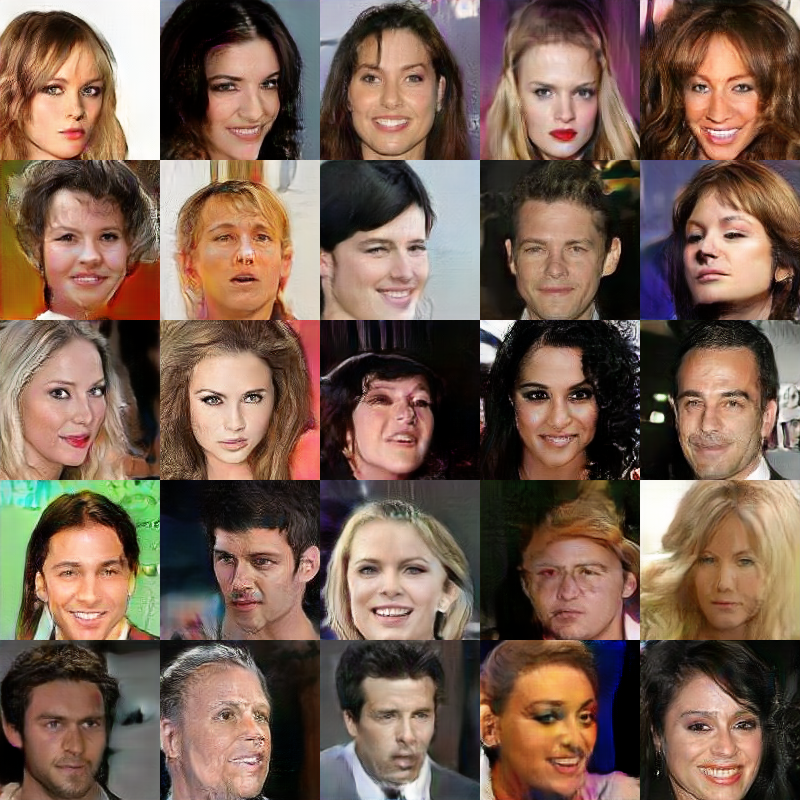
\includegraphics[width=.32\columnwidth]{samples/celeba-mmd-rq-25.png}
%      ~
%      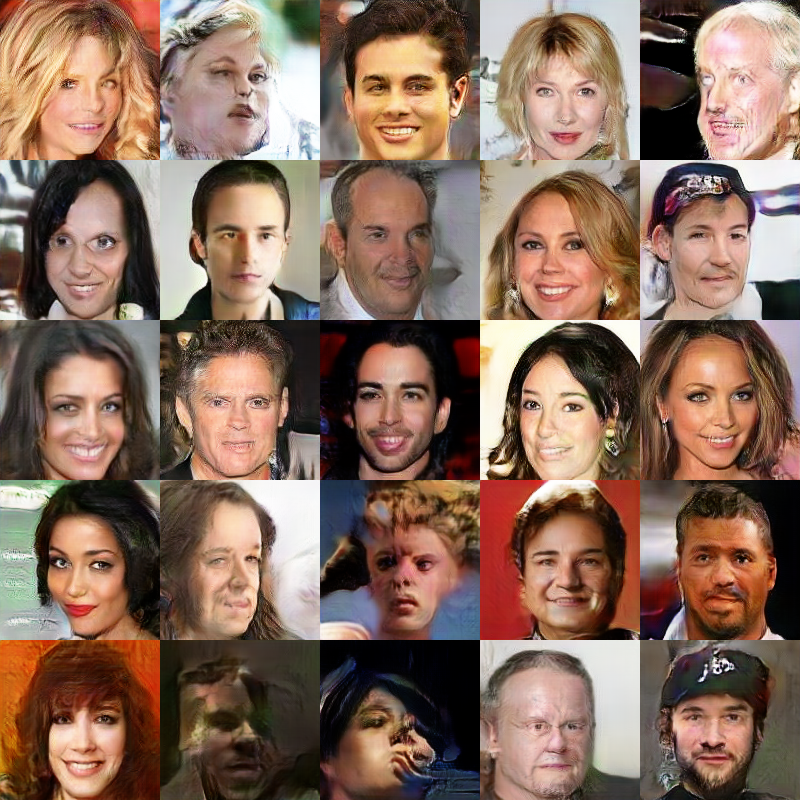
\includegraphics[width=.32\columnwidth]{samples/celeba-wgan-25.png}
%      ~
%      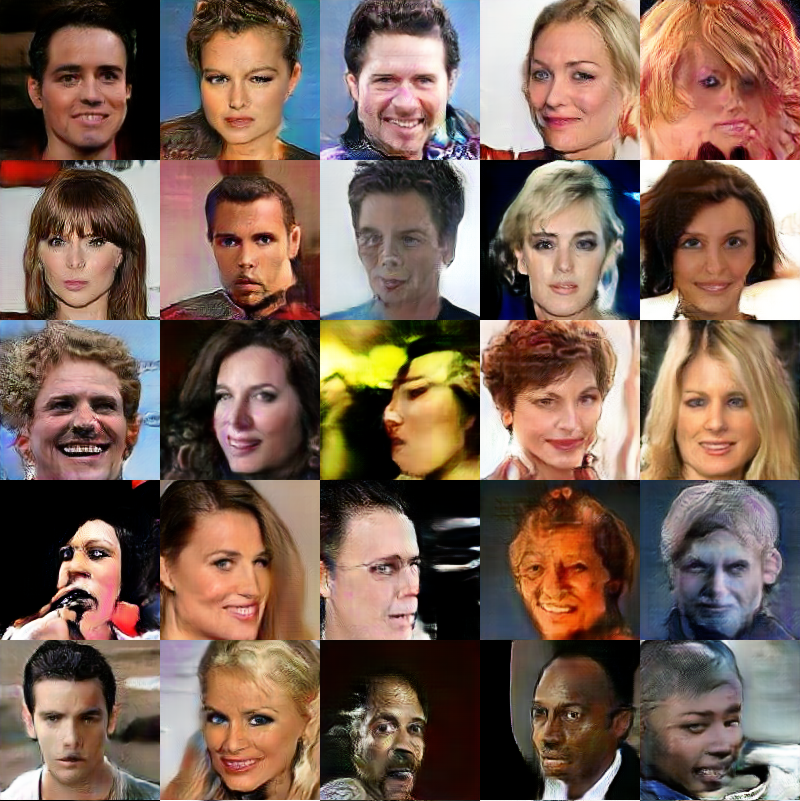
\includegraphics[width=.32\columnwidth]{samples/celeba-cramer-25.png}
%      \caption{Samples for \textbf{$160 \times 160$ CelebA} dataset trained with 
%               MMD GAN (left) and WGAN-GP (right) with ResNet generator and DCGAN discriminator.}
%    \end{figure}

    \begin{minipage}{.6\linewidth}
      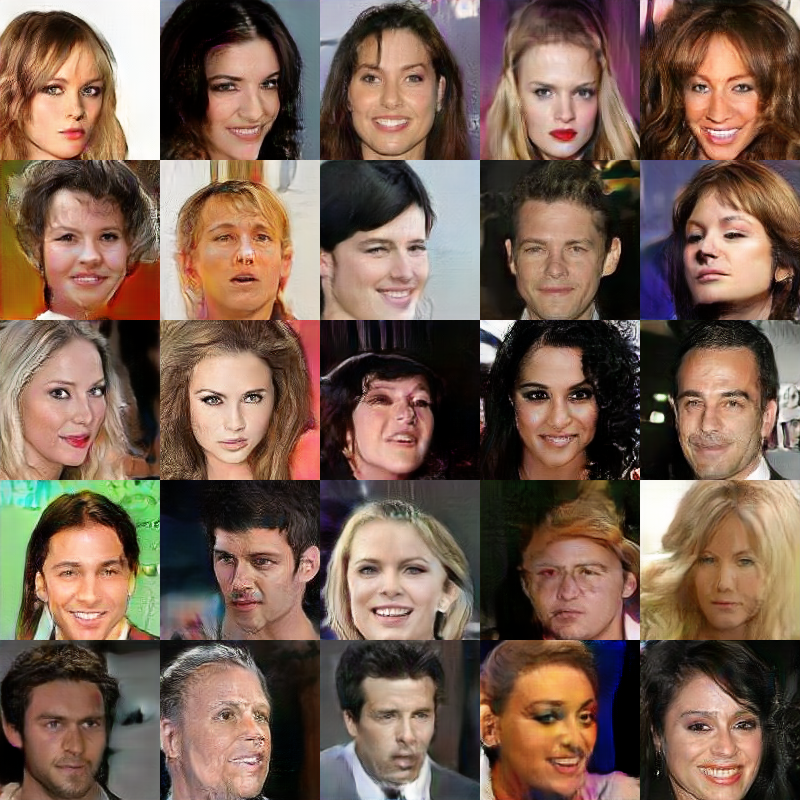
\includegraphics[width=.49\linewidth]{samples/celeba-mmd-rq-25.png}
      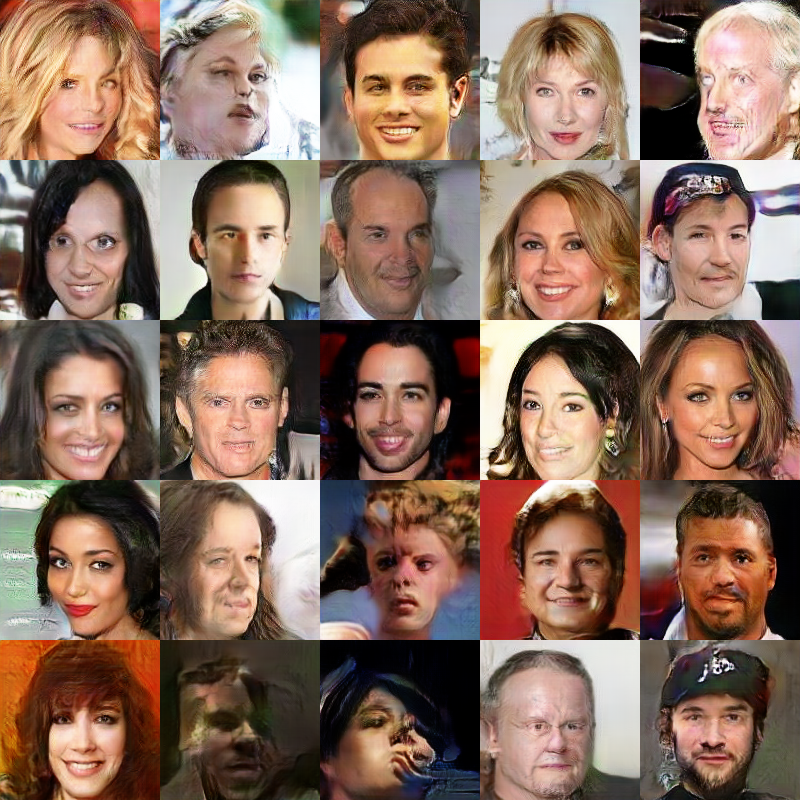
\includegraphics[width=.49\linewidth]{samples/celeba-wgan-25.png}
    \end{minipage}
    \begin{minipage}{.39\linewidth}
      \textbf{CelebA, $160 \times 160$.} \\
      MMD GAN (left) and WGAN-GP (right) samples,
      with ResNet generator and DCGAN critic.
    \end{minipage}

    \begin{minipage}{.6\linewidth}
      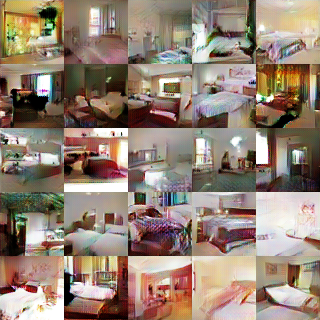
\includegraphics[width=.49\linewidth]{samples/lsun_rq_16.png}
      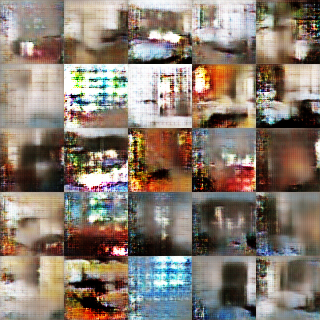
\includegraphics[width=.49\linewidth]{samples/lsun_wgan_16.png}
    \end{minipage}
    \begin{minipage}{.39\linewidth}
       \textbf{LSUN bedroom, $64 \times 64$.}\\
       MMD GAN (left) and WGAN-GP (right),
       with \emph{small critic} DCGANs ($4\times$ less convolutional filters).
    \end{minipage}
    ~\\

    CelebA scores (mean + standard deviation):
    % \begin{table}
    %   \centering
    %   \vspace{-1cm}
    %   \caption{Mean (standard deviation) of score evaluations for the CelebA dataset.}
    %   \label{tab:celeba-scores}
    \begingroup \renewcommand{\arraystretch}{1.1}
    \begin{tabular}{cc|rrr}
        loss & top layer & \multicolumn{1}{c}{Inception} & \multicolumn{1}{c}{FID} & \multicolumn{1}{c}{KID} \\
        \hline
        MMD RQ   &   16 &    2.61  (0.01) &   20.55  (0.25) &   0.013  (0.001)\\
        Cram\'er &  256 &    2.86  (0.01) &   31.30  (0.17) &   0.025  (0.001)\\
        WGAN-GP  & 1    &    2.72  (0.01) &   29.24  (0.22) &   0.022  (0.001)\\
        test set & --   &    3.76  (0.02) &    2.25  (0.04) &   0.000  (0.000)\\
    \end{tabular}
    \endgroup
  % \end{table}
  \end{column}

  \begin{column}{.32\textwidth}
    \begin{block}{New evaluation method: KID}
      Inception scores are independent of the target distribution;
      not meaningful for LSUN or CelebA.

      Fr\'echet Inception Distance (FID) \citep{fid} is better,
      but estimator is very biased:
      \vspace*{-1.5ex}\begin{itemize}
        \item Bias \emph{very} strong across sample sizes (figure below).
        \item 
        Easy to find models $\PP_1$, $\PP_2$ and target $\QQ$ where
        \[
          \FID(\PP_1, \QQ) < \FID(\PP_2, \QQ)
          \text{ but }
          \E \FID(\hat\PP_1, \QQ) > \E \FID(\hat\PP_2, \QQ)
        \]
        for reasonable sample sizes.
        \item Monte Carlo ``confidence intervals'' are meaningless.
      \end{itemize}

      Proposed \emph{Kernel Inception Distance} (KID):
      $\mmd^2$ estimate with kernel $k(x, y) = \left( x^{\mathsf T} y / d + 1 \right)^3$
      between Inception representations.
      \vspace*{-1.5ex}\begin{itemize}
        \item Similar to FID, but simple unbiased estimator.
        \item Estimator is computationally faster and needs fewer samples.
        \item Asymptotically normal: easy Monte Carlo confidence intervals.
      \end{itemize}

      FID (left) and KID (right) estimates between CIFAR-10 train and test sets.
      FID has strong bias and almost no variance;
      KID has no bias and rapidly decreasing variance.
      \\
      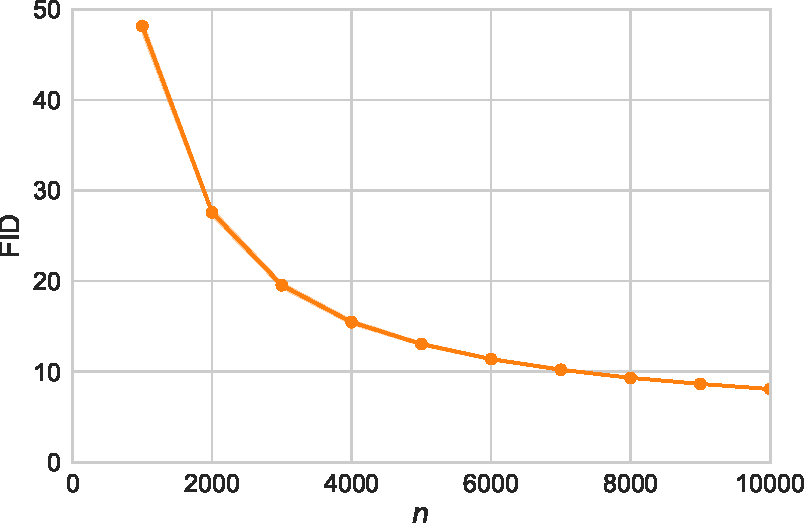
\includegraphics[width=.48\columnwidth]{figs/fid-bias.pdf}
      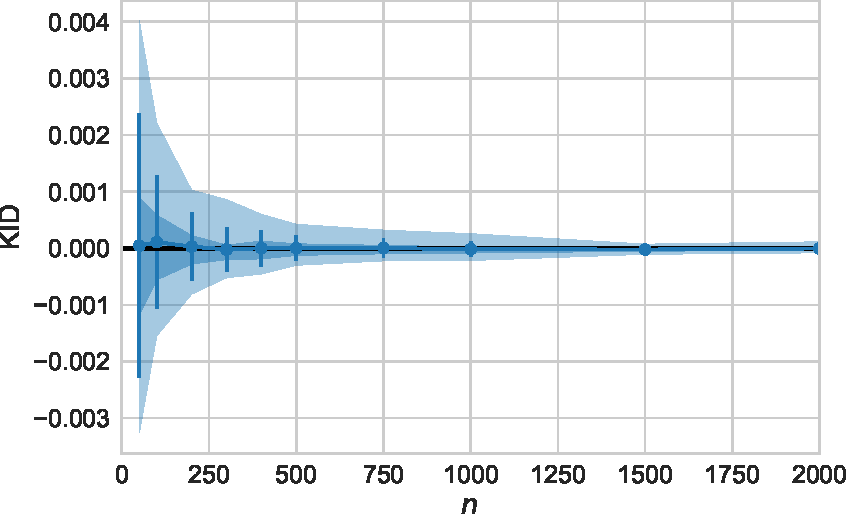
\includegraphics[width=.48\columnwidth]{figs/mmd-unbiased.pdf}
        % TODO: remake pictures the same size, and with bigger text...

        % \caption{Estimates of KID (left) and FID (right) between the CIFAR-10 train and test sets. FID estimates 
        %   exhibit strong bias for $n$ even up to $10\,000$, which is not the case for KID. 
        %   Standard deviation of estimates shrinks quickly for KID and is always small for FID.}  %Each point is based on 100 samples, estimating with replacement; sampling without replacement, and/or using the full training set, gives similar results. Lines show means, error bars standard deviations, dark colored regions a $\frac{2}{3}$ coverage interval of the samples, light colored regions a $95\%$ interval. Note the differing $n$ axes.}
        % \label{fig:fid-kid-bias}
    \end{block}

    \begin{block}{Learning Rate Adaptation}
      \begin{itemize}
%        \item Decreasing learning rate is common in deep learning.
        \item GAN learning rates usually tuned by hand; need to get it right.
        \item We propose an adaptive scheme: decrease if the KID score hasn't improved for a while, using an \emph{MMD relative similarity test} \citep{3sample}.
      \end{itemize}
    \end{block}

    \printbibliography
  \end{column}

\end{columns}


\end{frame}


\end{document}
